\documentclass{article}

\usepackage{arxiv}

\usepackage[utf8]{inputenc} % allow utf-8 input
\usepackage[T1]{fontenc}    % use 8-bit T1 fonts
\usepackage{hyperref}       % hyperlinks
\usepackage{url}            % simple URL typesetting
\usepackage{booktabs}       % professional-quality tables
\usepackage{amsfonts}       % blackboard math symbols
\usepackage{nicefrac}       % compact symbols for 1/2, etc.
\usepackage{microtype}      % microtypography
\usepackage{lipsum}
\usepackage{tcolorbox}
\usepackage{float}
\usepackage{graphicx}
\graphicspath{ {./images/} }
\usepackage[linesnumbered,ruled,vlined]{algorithm2e}

\title{Parallel Algorithms for Convex Hull}

\author{
  Kai Qin\\
  The University of Texas at Austin\\
  Austin, Texas \\
  \texttt{kai.qin@utexas.edu} \\
  %% examples of more authors
   \And
  Javier Valenzuela\\
  The University of Texas at Austin\\
  Austin, Texas \\
  \texttt{javier.valenzuela@utexas.edu} \\
}

\begin{document}
\maketitle

\begin{abstract}
This paper focuses on solving the 2D convex hull problem through parallel implementations. Given a set of 2D points, the goal is to find a subset which encloses the rest of the points and also is a convex polygon in shape. We describe the challenges and implementation details of two parallel convex hull algorithms: parallel MergeHull and parallel Monotone Chain convex hull. Our MergeHull is implemented using OpenMP and Monotone Chain convex hull is implemented using CUDA with Thrust library. The sequential algorithm presented as the baseline for correctness and performance is the Graham Scan algorithm. Experimental results shows that our CUDA implementation of the parallel Monotone Chain algorithm can achieve 10x speedups over baseline algorithm. Code for all implementations described on this paper can be found in the authors' repository\cite{repo}.
\end{abstract}

\section{INTRODUCTION}
The convex hull is a very basic problem in computational geometry, and many more complicated problems can be first reduced and then solved using an convex hull algorithm. It consists of, for a given set of points, finding the minimum set of points that enclose the whole set within a convex polygon(See Figure \ref{fig:example}). In recent history, the optimization of this problem has been crucial due to the huge spawn of applications in image analysis that make use of computational geometry algorithms, video game development, face recognition and navigation assistance for autonomous driving being the ones that stand out as applications the average person interacts with daily. These paper presents an attempt to replicate a small set of algorithms that solve this problem in parallel. CUDA was our first choice as the language for implementation due to its ability to directly render the results on the screen without sending back the results to the host CPU. OpenMP was also used as it facilitates implementation of recursive routines over CUDA, with a significant performance trade-off. Section 3 of this papers focuses on describing the different algorithms considered and detailing their implementation.

\begin{figure}[h]
\centering
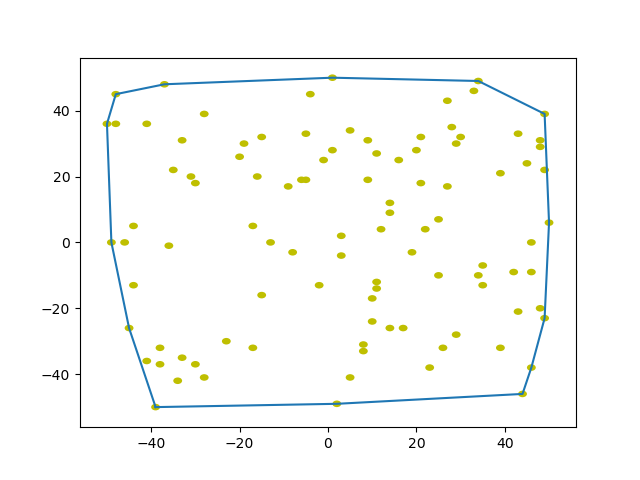
\includegraphics[scale=.4]{images/100_point_polygon.PNG}
\caption{Example of a convex hull for a set of 100 points}
\label{fig:example}
\end{figure}

\section{RELATED WORK}
The classical sequential Graham Scan algorithm convex hull algorithm \cite{Graham_72} first chooses a target point with smallest y-coordinate and sorts the input points by polar angle with the target point to get a simple polygon and consider points in the sorted order and discard those that would create a clockwise turn \cite{Graham_72}. Two parallel divide and conquer algorithms parallel QuickHull and MergeHull are introduced in \cite{blelloch1996parallel}. Both parallel QuickHull and MergeHull are expresses as recursive algorithms in \cite{blelloch1996parallel} and are named because their similarities to the QuickSort and MergeSort. QuickHull uses recursive function to handle each subsection of the input points. The recursion makes the algorithm easier to understand but more complex to optimize using CUDA where we need to spawn new threads from kernel rather than on the host. Srikanth \cite{srikanth2009parallelizing} introduced an Iterative 2D QuickHull which processes each subsection of the input points by providing labels to them according to extreme points of each segment. This idea of using labeling each segment by extreme points are also used in \cite{srungarapu2011fast}, \cite{tzeng2012finding}, \cite{Mei_2016}, and \cite{zhang2015novel}.

\section{Implementation Details}

\subsection{Graham Scan}

In the effort of having a sequential execution baseline to be used as reference for correctness and performance, the Graham Scan\cite{Graham_72} algorithm was chosen. This algorithm is a widely renown option for obtaining the convex hull of a set of points. One of the few requirements it has is that the data to be analyzed must be pre-sorted on a very specific order, choosing one point in the set as the source(typically the left most point or the lowest point) and sorting the rest of the points through the angle that they create with the source on the two-dimensional plane. Euclidean distance may be used as a tie breaker for points that form the same slope between vertices. The algorithm consists of traversing the set of points in the order previously established, and analyzing two pairs of points. Both of these pairs contain a point in common, which can be removed from the analysis whenever the two pairs have opposite orientation, breaking convexity.

\begin{algorithm}[H]
\SetAlgoLined
\KwIn{a set of input points $P$}
\KwOut{convex hull $H$}

\textit{Pre-sort data and assign leftmost point, called P0}\\
\For{$p$ in $P$}{
    \textit{pop the last point from the stack if we turn clockwise to reach this point}\\
    \While{count stack > 1 and ccw(next\_to\_top(stack), top(stack), $p$) < 0}
    {
        pop stack;
    }
    stack.push($p$);
}
return stack;
\caption{\textit{Graham_Scan(P)}}
\end{algorithm}

In the pseudo-code presented, $ccw$ represents a function that returns the orientation of the curve generated between three points, i.e, whether they are turning clock-wise or counter clockwise. Since every point is considered at least once, this algorithm has a time complexity of $O(n)$, although most literature will list it as $O(nlogn)$ accounting for the need to pre-sort the data. That step, as mention before, is omitted here. Multiple bibliographic sources and videos may be find online to visualize the progression of this algorithm, therefore, the explanation for this algorithm will be limited to focus on the parallel implementations considered.

\subsection{MergeHull}

This algorithm shares similarities with the MergeSort sorting algorithm, hence its similar name. The implementation of this code relies heavily on recursion, breaking the task of finding the convex hull into the smallest possible task. For this, there is a requirement for data to be massaged a certain way, such as in horizontal or vertical order. The implementation discussed on this paper considers points being sorted from left to right, with no two points being capable of having the same x value, to avoid running into a corner case where there is no area generated between any set of three points. Once the points are sorted, there are recursively split in half for their analysis, until they are broken down into sets of one or two points, in which case the resulting hull will be a point or a line, respectively. Once this is achieve, the computed hulls keep merging to one another in a similar fashion to that of a logarithmic reduction algorithm as the recursive routine resolves.

\begin{algorithm}[H]
\SetAlgoLined
\KwIn{a set of input points $P$}
\KwOut{convex hull $H$}
\uIf{$|P| < 3$}{return P;}
\Else{
$H_{left}$ := $MERGEHULL(P[0..|P|/2])$\;
$H_{rigth}$ := $MERGEHULL(P[|P|/2 +1 .. |P|-1])$\;
}
return $JOINHULLS(H_{left},H_{right}))$\;
\caption{\textit{MERGEHULL(P)}}
\end{algorithm}

\begin{algorithm}[H]
\SetAlgoLined
\KwIn{two vectors of points $H_l$ and $H_r$}
% \textit{// get left-most items in hulls}\\
% $indl = il = left\_most(Hl)$;\\
% $indr = ir = left\_most(Hr)$;\\
% \textit{// find upper tangent}\\
% $done = false$;\\
% \While{!done}{
%     $done = true$;\\
%     \While{$orientation(Hr[indr], Hl[indl], Hl[(indl + 1) \% Hl.size]$) = counter-clockwise}
%     {
%         $indl = (indl +1) \% Hl.size$; 
%     }
%     \While{$orientation(Hl[indl], Hr[indr], Hr[(Hr.size +indr - 1) \% Hr.size]$) = clockwise}
%     {
%         $indr = (indr +1) \% Hr.size$; 
%     }
% }
% $upperl = indl, upperr = indr$;\\
% \textit{// find lower tanget}\\
% $indl = il, indr = ir$;\\
% $done = false$;\\
% \While{!done}{
%     $done = true$;
%     \While{$orientation(Hl[indl], Hr[indr], Hr[(indr + 1) \% Hr.size]$) = counter-clockwise}
%     {
%         $indr = (indr +1) \% Hr.size$; 
%     }
%     \While{$orientation(Hr[indr], Hl[indl], Hl[(Hl.size +indl - 1) \% Hl.size]$) = clockwise}
%     {
%         $indr = (indr +1) \% Hl.size$; 
%     }
% }
% $lowerl = indl, lowerr = indr$;\\
find upper tangent and assign point to $upper_l$ and $upper_r$;\\
find lower tangent and assign point to $lower_l$ and $lower_r$;\\
$merged = empty\_vector()$;\\
\textit{// Merge both hulls into one using tangent points}\\
$ind = upper_l$; \\
$merged.add(H_l[upper_l])$; \\
\While{ind != lower_l}{
    $ind = (ind + 1)$ \% $H_l.size$;\\
    $merged.add(H_l[ind])$;
}
$ind$ = $lower_r$;\\
\While{ind != upper_r}{
    $ind = (ind + 1)$ \% $H_r.size$;\\
    $merged.add(H_r[ind])$;
}
return $merged$;
\caption{\textit{JOINHULLS($H_l$,$H_r$)}}
\end{algorithm}
The key challenge in implementing this algorithm rests in how to compute which points will be creating the upper and lower tangents between the two minor hulls, which describe the new route that will encompass the combined hull generated. This requires the traversal of the existing hulls, in which upper and lower boundaries for the tangents require the comparison of the area between the a point in one of the hulls and two points of the opposite hull. Once the are changes in polarity, it is known that an inflexion point is reached, an therefore, one of the boundaries. This is not an operation that can be done in constant time. Since all level of the reduction($O(log n)$) may result in the evaluation of points in an amount that varies with total number of points($O(n)$), it is concluded that the time complexity of this algorithm is of order $O(nlogn)$

\subsection{Parallel Monotone Chain Convex Hull}
As the OpenMP MergeHull is unable to achieve its ideal performance due to the lack of $n/2$ concurrent threads in our system, the foces of this paper switch into other convex hull algorithms that have been designed for CUDA. The basic idea of the sequential Monotone Chain convex hull algorithm is to first sort all the input points by their x-coordinate and then discard "non-extreme points"\cite{zhang2015novel}\cite{andrew1979another}. The sequential Monotone Chain constructs the convex hull in $O(nlogn)$ time, as it needs to sort the points first. The parallel implementation used for this paper is based on the algorithm given in \cite{zhang2015novel}. One primary reason this algorithm was chosen is that the paper clearly describes which Thrust operation that they choose for their implementation. Thrust is a C++ template library for CUDA based on the Standard Template Libray that provides a rich collection of data parallel primitives such as scan, sort, and reduce\cite{zhang2015novel}. Without the source code from the authors, some implementation details were missing from the given algorithms. Therefore, modifications were made to the original algorithm to help our implementation as shown in Algorithm \ref{cudahull}: Parallel Monotone Chain convex hull.

\begin{algorithm}[H]
\SetAlgoLined
\KwIn{a set of input points $P$}
\KwOut{convex hull $H$}
\textbf{First Split}\\
Use parallel reduction to find the leftmost point $P_{minx}$ and the rightmost point $P_{maxx}$\\
Determine the positions of the rest points against the line $P_{minx}P_{maxx}$\\
Assign a flag value to indicate the position: $flag =1$ when above or on the line and $flag=0$ when below the line but not on the line. \\
Use parallel partition to split the points into two segments according to the flag values: the lower subset $S_{lower}$ and the upper subset $S_{upper}$\\
Use parallel sorting to sort the $S_{lower}$ in $x$-ascending and $S_{upper}$ in $x$-descending\\
Update head, flags, keys, and first points, so that there are two segments $S_{lower}$ and $S_{upper}$\\
\textbf{Removing Interior Points Step}\\
\textbf{Repeat}\\
\For{each segment $(P_{first},P_{last})$ represented by two points $P_{first}$ and $P_{last}$ \textbf{in parallel}} {
  Find the fartheset point $P_{far}$ from the line $P_{first}P_{last}$\\
  Detect interior points by determining the positions with respect to $P_{first}$, $P_{last}$, and $P_{far}$ \\
  Assign each point a state flag depending on its position to indicate the state: 1: current non-interior points; 0: determined interior points\\
  Use parallel stable\_partition to gather all interior points according to the state flags, then remove all interior points\\
  Update all segments (including head flags, keys, first points) to divide segment $(P_{first}P_{last})$ into two new segments $(P_{first}P_{last})$ and $(P_{first}P_{last})$\\
}
\textbf{Until} there are no interior points can be found\\
\textbf{return} the remaining points in $P$ as the extreme points of $H$
\caption{\textit{Parallel CUDA Monotone Chain Convex Hull}}
\label{cudahull}
\end{algorithm}
In regards the data structure chosen (see the table in figure \ref{cudadata}), the x, y coordinates with other auxiliary information are stored in separate vectors, such as described by\cite{zhang2015novel}. This way, the host and device vector feature of the Thrust library can be fully utilized, without the need of manually allocating memory spaces and keeping track of the device memory allocations. 

In the "First Split" section of Algorithm \ref{cudahull}, from line 2 to line 7, the original set of input points is separated into two segments: the lower hull $S_{lower}$ and the upper hull $S_{upper}$ with reference to the line that connects the point with minimum x coordinate and the point with the maximum x-coordinate $P_{minx}P_{maxx}$. One implementation detail that is not explicitly covered from line 4 in the original algorithm is what flag value we should use for the points hat on the line $P_{minx}P_{maxx}$. The decision was made to assign $flag=1$ to points on the line which also includes $P_{minx}$ and $P_{maxx}$. Line 6 was also added into the algorithm, since the original algorithm does not explicitly address how to initialize all the auxiliary vectors (the head, flags, keys, and first points) that are used to keep track of the segments. When implementing the parallel partition on line 5 and parallel sorting on line 6, Thrust's make\_zip\_iterator function will bundle the x, y coordinates and other auxiliary vectors to keep their order in synchronization. This technique is found from the source of \cite{Mei_2016} which introduces another sorting-based preprocessing algorithm. \begin{figure}[H]
\centering
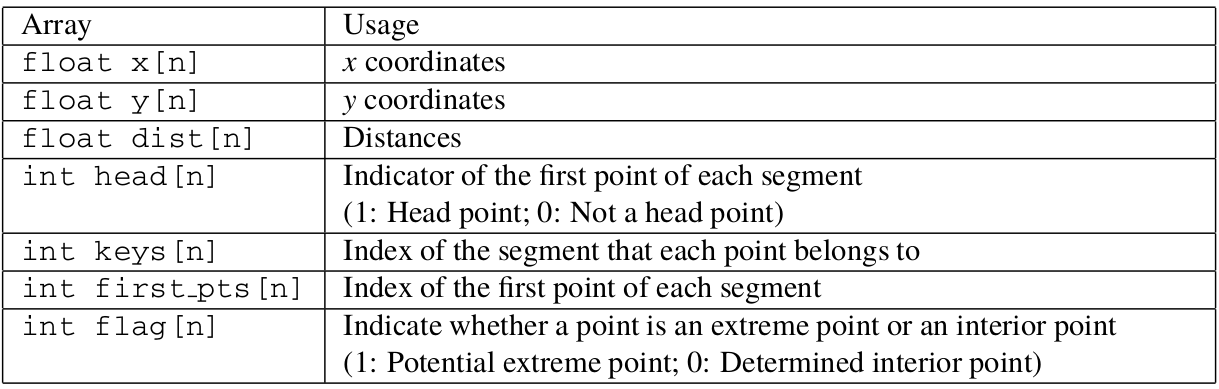
\includegraphics[scale=0.5]{images/cudatable.png}
\caption{Data structures for storing coordinates and auxiliary information. \cite{zhang2015novel}}
\label{cudadata}
\end{figure}

In the "Removing Interior Points Step", unlike QuickHull \cite{blelloch1996parallel} which handles each segment in each recursive call of the SUBHULL \cite{blelloch1996parallel} function, this algorithm performs each operation on each segment in parallel using segmented scan technique. On line line 11, the distance of each point to its corresponding first point and last point using is calculated a CUDA kernel designed by the authors, and then use Thrust::reduce\_by\_key function to find the maximum distance point $P_{far}$ and index of this point in each segment and store both in two temporary device vectors. Here we use another vector that stores the indices of the last points of each point in a segment before we run the CUDA kernel to calculate the distances of each points. On line 12, we use the same test for interior points as in \cite{zhang2015novel}. Assuming there is a triangle ABC from every segment, where A is $P_{first}$, C is $P_{last}$, and B is $P_{far}$. Since each point on each segment has been sorted according to their x-coordinate, the x-coordinates of point A, B and C can only be either ascending or descending. Since B is the point with the farthest distance from the line $(P_{first},P_{last})$, B can only be either to the left of the directed line AC or to the directed line CA depending on whether the segment is on the upper hull or the lower hull. Therefore, when B is to the left of the directed line AC, any point within the same segment is considered to be an determined interior point if is not outside the left side the directed line AB or outside the left side of the directed line BC. When B is to the left of the directed line CA, any point within the same segment is considered to be an determined interior point if is not outside the right side the directed line CB or outside the right side of the directed line BA.

In the original algorithm, all the segments including segment ids (variable keys[n]) of each segment are updated after we find the farthest point $P_{far}$ on line 11. This way, each old segment have been divided into two new segments and the interior point test needs to be conducted across two new consecutive segments, which requires more complicated kernels to perform segmented scan to run the triangular inclusion test we describe above. Therefore, in our implementation, this update is postponed until line 15. This way, during the interior point test, the old segment ids can still be used to test each point in each segment using its $(P_{first},P_{last})$ and $P_{far}$. 


\section{RESULTS}
 Experimentation was performed using a system with a i3-8100 processor (3.6GHz), 16GB of memory and a NVIDIA GeForce GTX1080 (Pascal Architecture) and CUDA compilation tools, release 11.0, V11.0.194, and GCC 9.2.1, and OPENMP 201511. 
Table \ref{runtable} shows a comparison of the execution times measured from the different implementations with sets of points of varying sizes randomly distributed in a square with side length of 500k pixels. The experimental results shows that our CUDA implementation of the parallel Monotone Chain algorithm can achieve 10x speedups over baseline algorithm with logarithmic increase over the input size.

It is interesting to note that the MergeHull algorithm shows worse average performance than that of the Graham Scan algorithm. The main conclusion that the authors reached to justify this behavior is the limited amount of parallelization that could be achieved with the system utilized for testing. Most general purpose CPUs have the capability of spawning up to a few tens of threads. This represents a challenge for MergeHull, as in its lowest recursion level, it requires up to $n/2$ concurrent threads to achieve its ideal performance. This number of threads is not achievable with CPUs and OpenMP, and ends up causing more harm than good. The parallel implementation represents a considerable amount of overhead in work, that is run in a quasi-sequential manner due to the reduced number of processors. For reproducing purposes, code for the implementations used can be found in $https://github.com/jvalenzuelaochoa/parallel-algs-finalProj$.


\begin{table}[]
\centering
\caption{Comparison of running time (/ms) for points distributed in a rectangle.}
\label{runtable}
\begin{tabular}{|c|c|c|c|}
\hline
No. of points & Graham Scan & MergeHull & Monotone Chain \\ \hline
1k            & 0.165       & 2         & 2.28           \\ \hline
10k           & 1.63        & 21        & 2.37           \\ \hline
100k          & 16.4        & 210       & 3.95           \\ \hline
200k          & 32.8        & 436       & 5.79           \\ \hline
500k          & 81.8        & 910       & 9.2            \\ \hline
600k          & 101.6       & 1193      & 9.02           \\ \hline
700k          & 114.2       & 1550      & 11.6           \\ \hline
800k          & 130.9       & 1795      & 12.2           \\ \hline
900k          & 152.2       & 1839      & 12.2           \\ \hline
1M            & 169.9       & 1921      & 14.8           \\ \hline
\end{tabular}
\end{table}
\section{CONCLUSION AND FUTURE WORK}
We have presented the challenges and implementation details of two parallel convex hull algorithms: parallel MergeHull and parallel Monotone Chain convex hull using OpenMP and CUDA. Our implementation of the parallel Monotone Chain algorithm validates the correctness and performance of the original algorithm and provides additional modifications that makes the algorithm easier to be implemented using CUDA. We have also evaluated the performance of our implementations using points randomly distributed in a square.

In \cite{zhang2015novel}, the authors also introduce a way of pre-processing the input points by first locating the 4 extreme points with minimum x, maximum x, minimum y, and maximum y, and then exclude input points inside the parallelogram formed by the 4 extreme points. Due to the time limitation, this technique could not be implemented and could be ont of the first items to revisit in the future. Another consideration can be done in regards to the observations made in the results section for the MergeHull algorithm, and capitalize on implementations that would allow for more simultaneous threads to assist in the divide and conquer approach that is presented. The most compelling option would be to work on a CUDA implementation, with the consideration that for larger data sets, the $n/2$ ideal requirement for the amount of threads may still be hard to obtain.

\bibliographystyle{unsrt}  
\bibliography{references}  %%% Remove comment to use the external .bib file (using bibtex).
%% and comment out the ``thebibliography'' section.

%% Comment out this section when you \bibliography{references} is enabled.
% \begin{thebibliography}{1}

% \bibitem{kour2014real}
% George Kour and Raid Saabne.
% \newblock Real-time segmentation of on-line handwritten arabic script.
% \newblock In {\em Frontiers in Handwriting Recognition (ICFHR), 2014 14th
%   International Conference on}, pages 417--422. IEEE, 2014.

% \end{thebibliography}

\end{document}

% \subsection{QuickHull}

% While we are implementing the parallel QuickHull algorithm from \cite{blelloch1996parallel} using CUDA, we realized that the major obstacle to achieving the acclaimed parallel speed-up is how to implement a recursive algorithm using CUDA. Based on our limited resources we found on how to implement recursive kernels using CUDA, we 

% Comparing to  our implementations of the sequential convex hull Graham Scan algorithm and QuickHull using OpenMP, we bundled together the x, y coordinates with auxiliary properties associated with each point.

% \begin{algorithm}[H]
% \SetAlgoLined
% \KwIn{a set of input points $P$}
% \KwOut{convex hull $H$}
% $X$ := ${x:(x,y) \in P}$\;
% $x_{min}$ := ${P(min_index(X)}$\;
% $x_{max}$ := ${P(max_index(X)}$\;
% return SUBHULL$(P, x_{min},x_{max})\cup$ SUBHULL$(P, x_{max},x_{min})$\;
% \caption{\textit{QUICKHULL(P)}}
% \end{algorithm}

% \begin{algorithm}[H]
% \SetAlgoLined
% $P'$:= $\{p \in P | \textrm{LEFT\_OF}?(p,(p_1,p_2))\}$\;
% \uIf{$|P'|<2$}{
%  return $p_1 \cup P'$\;
% } \Else {
%   $i$ := $\textrm{MAX\_INDEX}({\textrm{DISTANCE}(p,(p_1,p_2)): p \in P'})$\;
%   $p_m$ := $P'[i]$\;
%     \textbf{in parallel do:}\\
%     $H_l$ := $\textrm{SUBHULL}(P',p_1, p_m)$\;
%     $H_r$ := $\textrm{SUBHULL}(P',p_m, p_2)$\;
%     return $H_l \cup H_r$\;
% }
% \caption{\textit{SUBHULL(P,$p_1$,$p_2$)}}
% \end{algorithm}


% \begin{center}
%  \begin{tabular}{||c|c|c|c|c||} 
%  \hline
%  No. of points & Graham Scan  & MergeHull& Monotone Chain\\[0.5ex] 
%  \hline\hline
%  1E0 & 0  0 & 0 \\ 
%  \hline
%  1E1 & 0 & 0 & 0 & 0 \\ 
%  \hline
%  1E2 & 0 & 0 & 0.001 & .006\\
%  \hline
%  1E3 & 0 & 0 & 0.002 & .006 \\
%  \hline
%  1E4 & .001 & 0 & 0.021 & .007 \\
%  \hline
%  1E5 & .01 & 0 & 0.210 & .014 \\
%  \hline
%  1E6 & .104 & 0 & 1.921 & 0 \\
%  \hline
%  1E7 & 1.036 & 0 & 21.855 & 0 \\
%  \hline
%  1E8 & 10.065 & 0 & 265.759 & 0 \\ [1ex] 
%  \hline
% \end{tabular}
% \end{center}